%
%
\documentclass[twoside,11pt]{../sty/report_petsc}

\usepackage{makeidx,xspace}
\usepackage[bookmarksopen,colorlinks]{hyperref}
\usepackage[all]{hypcap}
\usepackage{color}
\input pdfcolor.tex     

\usepackage[pdftex]{graphicx}


\usepackage{times}
\usepackage{listings}
%\usepackage{psfig}
\usepackage{../sty/verbatim}
\usepackage{../sty/tpage}
\usepackage{../sty/here}
\usepackage{../sty/anlhelper}
\usepackage[hyphens,spaces,obeyspaces]{../sty/trl}
 
\setlength{\textwidth}{6.5in}
\setlength{\oddsidemargin}{0.0in}
\setlength{\evensidemargin}{0.0in}
\setlength{\textheight}{9.2in}
\setlength{\topmargin}{-.8in}

\newcommand{\findex}[1]{\index{#1}}
\newcommand{\sindex}[1]{\index{#1}}
\newcommand{\A}{\mbox{\boldmath \(A\)}}
\newcommand{\F}{\mbox{\boldmath \(F\)}}
\newcommand{\J}{\mbox{\boldmath \(J\)}}
\newcommand{\x}{\mbox{\boldmath \(x\)}}
\newcommand{\bb}{\mbox{\boldmath \(b\)}}
\newcommand{\rr}{\mbox{\boldmath \(r\)}}
hyperbaseurl

\makeindex
 
% Defines the environment where design issues are discussed. In the manual
% version of this report, these regions are ignored.
\def\design{\medskip \noindent Design Issue:\begin{em}}
\def\enddesign{\end{em} \medskip}
% Manual version:
% \def\design{\comment}
% \def\enddesign{\endcomment}

% Print DRAFT in large letters across every page
%\special{!userdict begin /bop-hook{gsave 200 70 translate
%65 rotate /Times-Roman findfont 216 scalefont setfont
%0 0 moveto 0.95 setgray (DRAFT) show grestore}def end}

% Defines that we're doing the whole manual, not the short intro part,
% used in part1.tex.
\def\shortintro{false}

\usepackage{fancyhdr,lastpage}
\pagestyle{fancy}
\rhead{PETSc 3.2 \today}

\begin{document}

%\pagestyle{empty}
%\begin{figure*}[hbt]
%\centerline{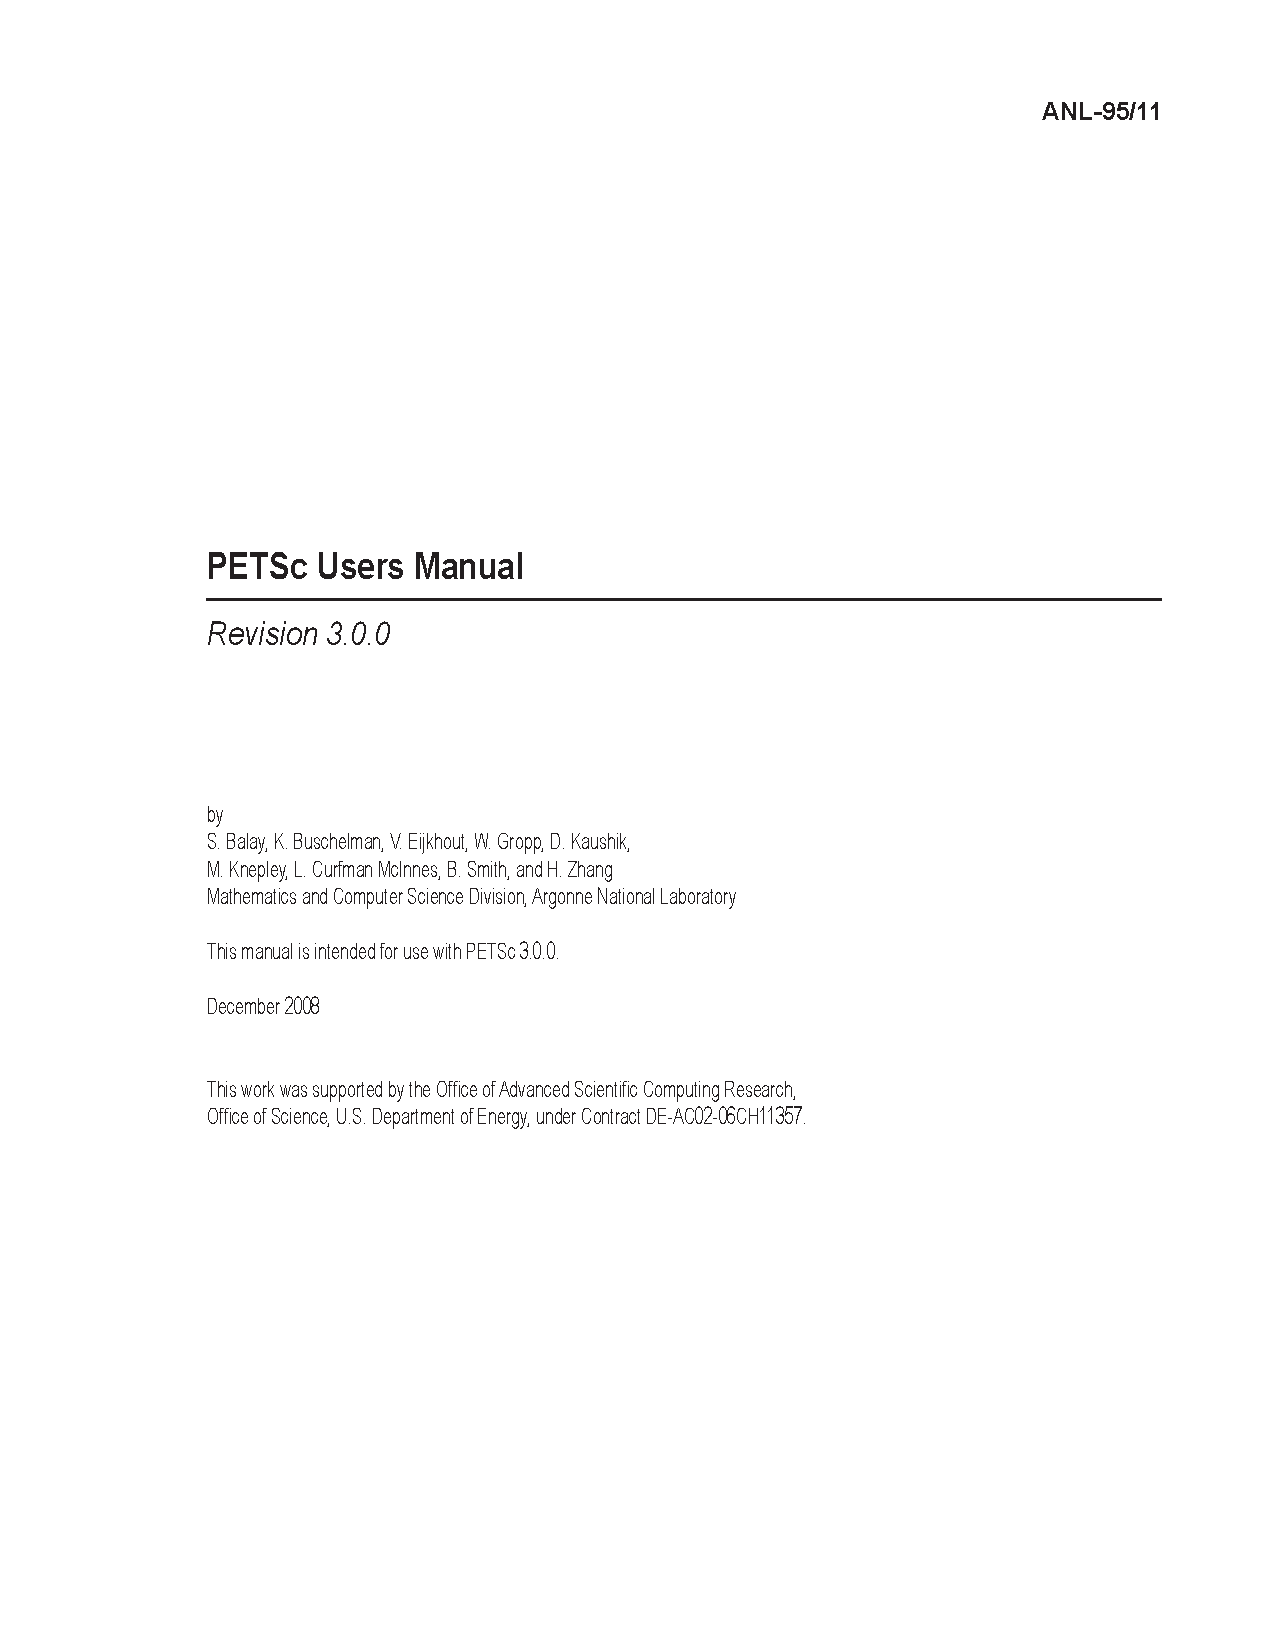
\includegraphics{titlepage1}}
%\end{figure*}

%  ANL changed the style of its title pages - so we are using titlepage1.pdf [above]
%  The following is an attempt to emulate titlepage1.pdf in latex

%%%%%%%%%%%%%%%%%%%%%%%%%%%%%%%%%%%%%%%%%%%%%%%%%%%%%%%%%%%%%%%%%%%%%%%%%%%%%%%%%%%%

\hfill {\large{\bf ANL-95/11}}

\vspace*{3in}
\noindent {\huge{\bf PETSc Users Manual}}
\vspace*{8pt}
\hrule
\vspace*{8pt}
\noindent {\huge{\it Revision 3.2}}

\vspace*{1in}
\noindent by \\
S. Balay, J. Brown, K. Buschelman, V. Eijkhout, W. Gropp, D. Kaushik, \\
M. Knepley, L. Curfman McInnes, B. Smith, and H. Zhang \\
Mathematics and Computer Science Division, Argonne National Laboratory

\vspace*{10pt}
\noindent Sept 2011

\vspace*{20pt}
\noindent This work was supported by the Office of Advanced Scientific Computing Research, \\
Office of Science, U.S. Department of Energy, under Contract DE-AC02-06CH11357.

%%%%%%%%%%%%%%%%%%%%%%%%%%%%%%%%%%%%%%%%%%%%%%%%%%%%%%%%%%%%%%%%%%%%%%%%%%%%%%%%%%%%

\begin{figure*}[hbt]
\centerline{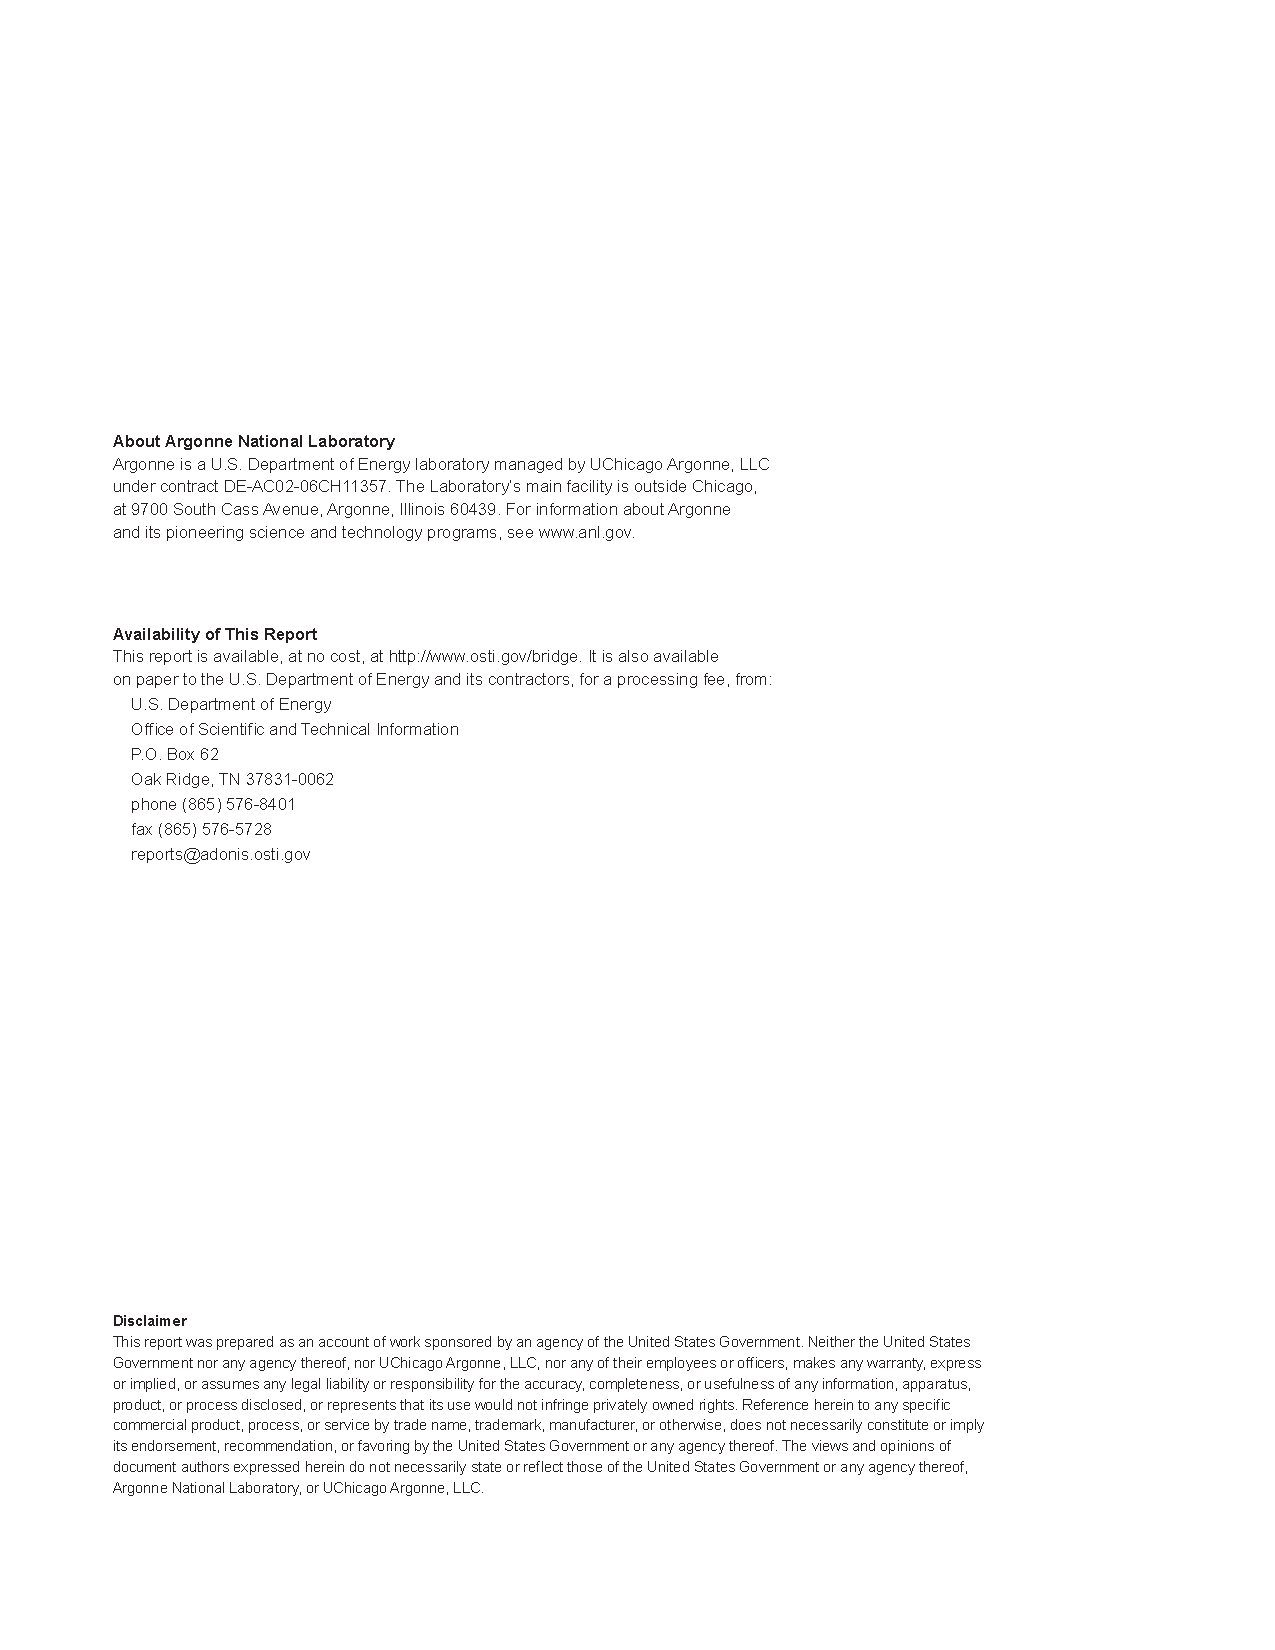
\includegraphics{titlepage2}}
\caption{}
\end{figure*}


\cleardoublepage
%\pagestyle{plain}

\vspace{1in}
\date{\today}

% Abstract for users manual
\addcontentsline{toc}{chapter}{Abstract}
% Abstract for PETSc Users Manual

%
%   Next line temp removed
%
\noindent {\bf Abstract:} 

\medskip \medskip
This manual describes the use of PETSc for the numerical solution
of partial differential equations and related problems 
on high-performance computers.  The
Portable, Extensible Toolkit for Scientific Computation (PETSc) is a
suite of data structures and routines that provide the building
blocks for the implementation of large-scale application codes on parallel
(and serial) computers.  PETSc uses the MPI standard for all
message-passing communication.

PETSc includes an expanding suite of parallel linear, nonlinear
equation solvers and time integrators that may be
used in application codes written in Fortran, C, C++, and Python.  PETSc
provides many of the mechanisms needed within parallel application
codes, such as parallel matrix and vector assembly routines. The library is
organized hierarchically, enabling users to employ the level of
abstraction that is most appropriate for a particular problem. By
using techniques of object-oriented programming, PETSc provides
enormous flexibility for users.

PETSc is a sophisticated set of software tools; as such, for some
users it initially has a much steeper learning curve than a simple
subroutine library. In particular, for individuals without some
computer science background, experience programming in C, C++ or Fortran and experience using a debugger such as \trl{gdb} or \trl{dbx}, it
may require a significant amount of time to take full advantage of the
features that enable efficient software use.  However, the power of
the PETSc design and the algorithms it incorporates may make the efficient
implementation of many application codes simpler than ``rolling
them'' yourself.
\begin{itemize}
\item  For many tasks a package such as MATLAB is often the best tool; PETSc is not
intended for the classes of problems for which effective MATLAB code
can be written.
\item PETSc should not be used to attempt to provide
a ``{\bf parallel linear solver}'' in an otherwise sequential code.
Certainly all parts of a previously sequential code need not be parallelized but the 
matrix generation portion must be parallelized to expect any kind of reasonable performance.
Do not expect to generate your matrix sequentially and then ``use PETSc'' to solve
the linear system in parallel.
\end{itemize}

Since PETSc is under continued development, small changes in usage and
calling sequences of routines will occur.  PETSc is supported; see the
web site \href{http://www.mcs.anl.gov/petsc}{http://www.mcs.anl.gov/petsc} for information on
contacting support.

A \href{http://www.mcs.anl.gov/petsc/petsc-as/publications}{http://www.mcs.anl.gov/petsc/petsc-as/publications} may be found 
a list of publications and web sites that feature work involving PETSc.


We welcome any reports of corrections for this document.

\medskip \medskip





\cleardoublepage


% ---------------------------------------------------------------------------
%

\medskip\medskip

\noindent {\bf Getting Information on PETSc:} 

\medskip


\noindent {\bf On-line:}
\begin{list}{$\bullet$}
{
\setlength{\itemsep}{-.020in} 
\setlength{\topsep}{0in} 
\setlength{\partopsep}{0in}
}
\item Manual pages--example usage
\href{index.html}{docs/index.html}  or
\href{http://www.mcs.anl.gov/petsc/documentation}{http://www.mcs.anl.gov/petsc/documentation}
\item Installing PETSc
\href{http://www.mcs.anl.gov/petsc/documentation/installation.html}{http://www.mcs.anl.gov/petsc/documentation/installation.html}
\end{list}

\medskip
\noindent {\bf In this manual:}
\begin{list}{$\bullet$}
{
\setlength{\itemsep}{-.02in} 
\setlength{\topsep}{.02in} 
\setlength{\partopsep}{0in}
}
\item Basic introduction, page \pageref{sec_gettingstarted}
\item Assembling vectors, page \pageref{sec_vecbasic}; and matrices, \pageref{chapter_matrices}
\item Linear solvers, page \pageref{ch_ksp}
\item Nonlinear solvers, page \pageref{chapter_snes}
\item Timestepping (ODE) solvers, page \pageref{chapter_ts}
\item Index, page \pageref{ch_index}
\end{list}

% ---------------------------------------------------------------------------


\medskip \medskip

\cleardoublepage

% Acknowledgements for users manual
% Acknowledgements for PETSc Users Manual
%
%   this information is a DUPLICATE of misc/acknwldg.htm
%                MAKE SURE THEY MATCH!!!
%
\noindent {\bf Acknowledgments:}

\medskip \medskip \noindent
We thank all PETSc users for their many suggestions, bug reports, and
encouragement.  We especially thank David Keyes
for his valuable comments on the source code,
functionality, and documentation for PETSc.


\vspace{.3in}
\noindent
Some of the source code and utilities in PETSc
have been written by 
\begin{itemize}
  \item Asbjorn Hoiland Aarrestad - the explicit Runge-Kutta implementations;
  \item Mark Adams - scalability features of MPIBAIJ matrices;
  \item G. Anciaux and J. Roman - the interfaces to the partitioning packages Jostle, Scotch, Chaco, and Party;
  \item Allison Baker - the flexible GMRES code and LGMRES;
  \item Chad Carroll - Win32 graphics;
  \item Cameron Cooper - portions of the VecScatter routines;
  \item Paulo Goldfeld - balancing Neumann-Neumann preconditioner;
  \item Matt Hille;
  \item Joel Malard - the BICGStab(l) implementation;
  \item Dave May - the GCR implementation
  \item Peter Mell - portions of the DA routines;
  \item Richard Mills - the AIJPERM matrix format for the Cray X1 and universal F90 array interface;
  \item Victor Minden - the NVidia GPU interface;
  \item Todd Munson - the LUSOL (sparse solver in MINOS) interface and several Krylov methods;
  \item Adam Powell - the PETSc Debian package, 
  \item Robert Scheichl - the MINRES implementation,
  \item Karen Toonen - designed and implemented much of the PETSc web pages,
  \item Liyang Xu - the interface to PVODE (now Sundials/CVODE).
\end{itemize}

\vspace{.3in}
\noindent
PETSc uses routines from 
\begin{itemize}
  \item BLAS;
  \item LAPACK;
  \item LINPACK -    dense matrix factorization and solve; converted to C using {\tt f2c} and then 
                     hand-optimized for small matrix sizes, for block matrix data structures;
  \item MINPACK -    see page \pageref{sec_fdmatrix}, sequential matrix coloring routines for finite difference Jacobian
                     evaluations; converted to C using {\tt f2c};
  \item SPARSPAK -   see page \pageref{sec_factorization}, matrix reordering routines, converted to C using {\tt f2c};
  \item libtfs     - the efficient, parallel direct solver developed by Henry Tufo and Paul Fischer for the direct solution of a coarse grid problem (a linear system with very few degrees of freedom per processor).
\end{itemize}


\vspace{.3in}
\noindent
PETSc interfaces to the following external software:
\begin{itemize}
  \item ADIC/ADIFOR -  automatic differentiation for the computation of sparse Jacobians,\\ 
                     \href{http://www.mcs.anl.gov/adic}{http://www.mcs.anl.gov/adic},
                     \href{http://www.mcs.anl.gov/adifor}{http://www.mcs.anl.gov/adifor},
  \item AMG -         the algebraic multigrid code of John Ruge and Klaus Stueben,
                     \href{http://www.mgnet.org/mgnet-codes-gmd.html}{http://www.mgnet.org/mgnet-codes-gmd.html}
  \item BLOPEX - Block Locally Optimal Preconditioned Eigenvalue Xolvers developed by Andrew Knyazev,
                    \href{http://www-math.cudenver.edu/~aknyazev/software/BLOPEX/},
  \item Chaco -     A graph partitioning package, \href{ http://www.cs.sandia.gov/CRF/chac.html}{ http://www.cs.sandia.gov/CRF/chac.html}
  \item DSCPACK -    see page \pageref{sec_externalsol}, Domain-Separator Codes for solving sparse symmetric
                      positive-definite systems, 
                     developed by Padma Raghavan,   
                     \href{http://www.cse.psu.edu/~raghavan/Dscpack/}{http://www.cse.psu.edu/~raghavan/Dscpack/},
  \item ESSL -         IBM's math library for fast sparse direct LU factorization,
  \item Euclid  -   parallel ILU(k) developed by David Hysom, accessed through the Hypre interface,
  \item Hypre -    the LLNL preconditioner library, \href{http://www.llnl.gov/CASC/hypre}{http://www.llnl.gov/CASC/hypre}
  \item Jostle -     A graph partitioning package, \href{http://www.gre.ac.uk/~c.walshaw/jostle/}{http://www.gre.ac.uk/~c.walshaw/jostle/}
  \item LUSOL -       sparse LU factorization code (part of MINOS) developed by Michael Saunders,
                      Systems Optimization Laboratory, Stanford University,
                     \href{http://www.sbsi-sol-optimize.com/}{http://www.sbsi-sol-optimize.com/},
  \item Mathematica -  see page \pageref{ch_mathematica},
  \item MATLAB -      see page \pageref{ch_matlab},
  \item MUMPS -      see page \pageref{sec_externalsol}, MUltifrontal Massively Parallel sparse direct Solver developed by Patrick Amestoy, 
                     Iain Duff, Jacko Koster, and Jean-Yves L'Excellent, \\
                     \href{http://www.enseeiht.fr/lima/apo/MUMPS/credits.html}{http://www.enseeiht.fr/lima/apo/MUMPS/credits.html},
  \item ParMeTiS -     see page \pageref{sec_partitioning}, parallel graph partitioner,
                     \href{http://www-users.cs.umn.edu/~karypis/metis/}{http://www-users.cs.umn.edu/~karypis/metis/},
  \item Party -     A graph partitioning package, \\ \href{http://www.uni-paderborn.de/fachbereich/AG/monien/RESEARCH/PART/party.html}{http://www.uni-paderborn.de/fachbereich/AG/monien/RESEARCH/PART/party.html},
  \item PaStiX -     Parallel LU and Cholesky solvers,
  \item Prometheus - Scalable unstructured finite element solver \href{http://www.columbia.edu/~ma2325/prometheus/}{http://www.columbia.edu/~ma2325/prometheus/},
  \item PLAPACK - Parallel Linear Algebra Package, \href{http://www.cs.utexas.edu/users/plapack/}{http://www.cs.utexas.edu/users/plapack/},
  \item Scotch -     A graph partitioning package, \href{http://www.labri.fr/Perso/~pelegrin/scotch/}{http://www.labri.fr/Perso/~pelegrin/scotch/}
  \item SPAI -        for parallel sparse approximate inverse preconditiong, 
                     \href{http://www.sam.math.ethz.ch/~grote/spai/}{http://www.sam.math.ethz.ch/~grote/spai/},
  \item SPOOLES - see page \pageref{sec_externalsol}, SParse Object Oriented Linear Equations Solver, developed by Cleve Ashcraft, 
                    \href{http://www.netlib.org/linalg/spooles/spooles.2.2.html}{http://www.netlib.org/linalg/spooles/spooles.2.2.html},
  \item Sundial/CVODE - see page \pageref{sec_sundials}, parallel ODE integrator,
                     \href{http://www.llnl.gov/CASC/sundials/}{http://www.llnl.gov/CASC/sundials/},
  \item SuperLU and SuperLU\_Dist - see page \pageref{sec_externalsol}, 
                    the efficient sparse LU codes developed by Jim Demmel,  Xiaoye S. Li, and John Gilbert, 
                    \href{http://www.nersc.gov/~xiaoye/SuperLU}{http://www.nersc.gov/~xiaoye/SuperLU},
  \item Trilinos/ML - Sandia's main multigrid preconditioning package, \href{http://software.sandia.gov/trilinos/}{http://software.sandia.gov/trilinos/},
  \item UMFPACK - see page \pageref{sec_externalsol}, 
                    developed by Timothy A. Davis, 
                    \href{http://www.cise.ufl.edu/research/sparse/umfpack/}{http://www.cise.ufl.edu/research/sparse/umfpack/}.
\end{itemize}
These are all optional packages and do not need to be installed to use PETSc.

PETSc software is developed and maintained with 
\begin{itemize}
\item \href{http://mercurial.selenic.com/}{Mecurial} revision control system
\item Emacs editor
\end{itemize}

PETSc documentation has been generated using
\begin{itemize}
\item the \href{http://www.cs.uiuc.edu/~wgropp/projects/software/sowing/index.htm}{text processing tools} developed by Bill Gropp
\item c2html
\item pdflatex
\item python
\end{itemize}



% Blank page makes double sided printout look bettter.

\cleardoublepage

\tableofcontents

% --------------------------------------------------------------------
%                            PART 1
% --------------------------------------------------------------------
\cleardoublepage
\part{Introduction to PETSc}
\label{part_intro}
\cleardoublepage
\chapter{Getting Started}
\input{part1tmp.tex}

% --------------------------------------------------------------------
%                            PART 2
% --------------------------------------------------------------------
\cleardoublepage
\part{Programming with PETSc}
\label{part_usage}
\input{part2tmp.tex}


%------------------------------------------------------------------


\cleardoublepage
\bibliographystyle{plain}
\addtocounter{chapter}{1}
\addcontentsline{toc}{chapter}{Bibliography}
\label{sec:bib}
\bibliography{../petsc,../petscapp}

\pagestyle{empty}
\begin{figure*}[hbt]
\centerline{
\includegraphics{endpage}}
\caption{}
\end{figure*}

\end{document}


